%%%%%%%%%%%%%%%%%%%%%%%%%%%%%%%%%%%%%%%%%
% Masters/Doctoral Thesis 
% LaTeX Template
% Version 1.43 (17/5/14)
%
% This template has been downloaded from:
% http://www.LaTeXTemplates.com
%
% Original authors:
% Steven Gunn 
% http://users.ecs.soton.ac.uk/srg/softwaretools/document/templates/
% and
% Sunil Patel
% http://www.sunilpatel.co.uk/thesis-template/
%
% License:
% CC BY-NC-SA 3.0 (http://creativecommons.org/licenses/by-nc-sa/3.0/)
%
% Note:
% Make sure to edit document variables in the Thesis.cls file
%
%%%%%%%%%%%%%%%%%%%%%%%%%%%%%%%%%%%%%%%%%

%----------------------------------------------------------------------------------------
%	PACKAGES AND OTHER DOCUMENT CONFIGURATIONS
%----------------------------------------------------------------------------------------

\documentclass[11pt, oneside]{Thesis} % The default font size and one-sided printing (no margin offsets)

\graphicspath{{Pictures/}} % Specifies the directory where pictures are stored

\usepackage[spanish]{babel}

\usepackage{bmpsize}

\usepackage{booktabs}% http://ctan.org/pkg/booktabs
\newcommand{\tabitem}{~~\llap{\textbullet}~~}

\usepackage{float}
\usepackage{url}
\usepackage[square, numbers, comma, sort&compress]{natbib} % Use the natbib reference package - read up on this to edit the reference style; if you want text (e.g. Smith et al., 2012) for the in-text references (instead of numbers), remove 'numbers' 
\hypersetup{urlcolor=black, colorlinks=true} % Colors hyperlinks in blue - change to black if annoying
\title{\ttitle} % Defines the thesis title - don't touch this

\begin{document}

\frontmatter % Use roman page numbering style (i, ii, iii, iv...) for the pre-content pages

\setstretch{1.3} % Line spacing of 1.3

% Define the page headers using the FancyHdr package and set up for one-sided printing
\fancyhead{} % Clears all page headers and footers
\rhead{\thepage} % Sets the right side header to show the page number
\lhead{} % Clears the left side page header

\pagestyle{fancy} % Finally, use the "fancy" page style to implement the FancyHdr headers

\newcommand{\HRule}{\rule{\linewidth}{0.5mm}} % New command to make the lines in the title page

% PDF meta-data
\hypersetup{pdftitle={\ttitle}}
\hypersetup{pdfsubject=\subjectname}
\hypersetup{pdfauthor=\authornames}
\hypersetup{pdfkeywords=\keywordnames}

%----------------------------------------------------------------------------------------
%	TITLE PAGE
%----------------------------------------------------------------------------------------

\begin{titlepage}
\begin{center}
\textsc{\LARGE \univname}\\[1.5cm] % University name


\begin{figure}[htbp]
	\centering
		
\includegraphics[width=0.4\textwidth]{Figures/logo.png}
		\rule{35em}{0.5pt}
\end{figure}


\textsc{\Large Pŕactica Professional Supervisada de Ingeniería en Computación}\\[0.5cm] % Thesis type

\HRule \\[0.4cm] % Horizontal line
{\huge \bfseries \ttitle}\\[0.4cm] % Thesis title
\HRule \\[1cm] % Horizontal line
 
\begin{minipage}[t]{0.4\textwidth}
\begin{flushleft} \large
\emph{Autor:}\\
{\authornames}\\ % Author name - remove the \href bracket to remove the link
\emph{Matrícula:}35.104.714
\end{flushleft}
\end{minipage}
\begin{minipage}[t]{0.4\textwidth}
\begin{flushright} \large
\emph{Tutor Docente:} 
\\{Mg.Ing. Miguel \textsc{Solinas} }\\ % Supervisor name - remove the \href bracket to remove the link  
\emph{Supervisor:} \\
{\supname}\\~\\~\\ % Supervisor name - remove the \href bracket to remove the link  
\end{flushright}
\end{minipage}

\facname\\\groupname\\~\\ % Research group name and department name
 
{\large \today}\\ % Date
%\includegraphics{Logo} % University/department logo - uncomment to place it
\vfill
\end{center}
\end{titlepage}

\clearpage % Start a new page

%----------------------------------------------------------------------------------------
%	ABSTRACT PAGE
%----------------------------------------------------------------------------------------
\newpage

%----------------------------------------------------------------------------------------
%	LIST OF CONTENTS/FIGURES/TABLES PAGES
%----------------------------------------------------------------------------------------

\pagestyle{fancy} % The page style headers have been "empty" all this time, now use the "fancy" headers as defined before to bring them back

\lhead{\emph{Contenido}} % Set the left side page header to "Contents"
\tableofcontents % Write out the Table of Contents

\lhead{\emph{Lista de Figuras}} % Set the left side page header to "List of Figures"
\listoffigures % Write out the List of Figures

%\lhead{\emph{Lista de Tablas}} % Set the left side page header to "List of Tables"
%\listoftables % Write out the List of Tables

%----------------------------------------------------------------------------------------
%	ABBREVIATIONS
%----------------------------------------------------------------------------------------

\clearpage % Start a new page

\setstretch{1.5} % Set the line spacing to 1.5, this makes the following tables easier to read

%\lhead{\emph{Abreviaturas}} % Set the left side page header to "Abbreviations"
%\listofsymbols{ll} % Include a list of Abbreviations (a table of two columns)
%{
%\textbf{IEEE} & \textbf{I}nstitute of \textbf{E}lectrical and \textbf{E}lectronics \textbf{E}ngineers\\
%\textbf{SO} & \textbf{S}istema \textbf{O}perativo  \\
%\textbf{KDS} & \textbf{K}inetis \textbf{D}esign \textbf{S}tudio \\
%%\textbf{Acronym} & \textbf{W}hat (it) \textbf{S}tands \textbf{F}or \\
%}


%----------------------------------------------------------------------------------------
%	THESIS CONTENT - CHAPTERS
%----------------------------------------------------------------------------------------

\mainmatter % Begin numeric (1,2,3...) page numbering

\pagestyle{fancy} % Return the page headers back to the "fancy" style

% Include the chapters of the thesis as separate files from the Chapters folder
% Uncomment the lines as you write the chapters

% Chapter Template

\chapter{Introducción} % Main chapter title

\label{Chapter1} % Change X to a consecutive number; for referencing this chapter elsewhere, use \ref{ChapterX}

\lhead{Capítulo 1. \emph{Introducción}} % Change X to a consecutive number; this is for the header on each page - perhaps a shortened title

\section{Motivación y Objetivos}
Como primera parte de la práctica profesional se propuso el estudio y el análisis de arquitecturas y patrones de diseño empleados en el desarrollo de sistemas de software orientados a multiplataformas (o sistemas operativos) y con una fuerte influencia de frameworks de desarrollo.
Con esta tarea en mente se procedió a cumplir con las siguientes metas:

\begin{itemize}
	\item Entnender el concepto de patron de arquitectura de software
	\item Entender el concepto de patrones de diseño de software.
	\item Investigar las arquitecturas más comunmente usadas en el desarrollo de aplicaciones nativas para dispositivos móviles.
	\item Entender los detalles de las opciones y tomar en consideración las dificultades más importantes de cada alternativa.
	\item Elegir una opción y justificar tal elección
	\item Introducir una posible alterativa de implementación de tal arquitectura y la correspondiente descripción de componentes.
	 
\end{itemize}

En una segunda parte se analizará una implementación real del diseño expuesto.

\section{Sobre los patrones en la etapa de diseño}
El empleo de patrones de arquitectura así como patrones de diseño en el proceso de desarrollo de software permite estandarizar la abstracción del problema y modularizar la solución en componentes conocidos y de responsabilidad limitada. Definir una cantidad y variedad limitada de componentes favorece la reutilización de estructuras y tanto la implementación de nuevas funcionalidades así como la corrección de errores implica una ordenada cantidad de tareas que facilitan al mismo tiempo su apropiada planificación.
Tanto la manipulación de datos como la interacción con sistemas vecinos puede incorporarse como partes del diseño contemplado siempre y cuando se respete el esquema de responsabilidades y las políticas de dependencias.
Por lo general la utilización de patrones en la etapa de diseño ayuda a definir con precisión la distribución de responsabilidades entre distintas clases, incrementa la cohesión entre objetos, el encapsulamiento y la definición de contratos mediante la abstracción de interfaces.
Adicionalmente la inclusión de diseño como la inversión de control deberían facilitar en gran medida el planteo, la implementación y la ejecución de pruebas unitarias, funcionales y de interfaz de usuario.




%----------------------------------------------------------------------------------------
%	SECTION 1
%----------------------------------------------------------------------------------------

\section{Porqué invertir en una arquitectura sólida}
Una de las más comunes e incorrectas prácticas en el desarrollo de software es optar por utilizar un enfoque NAIVE (ingénuo) que permite ciertamente conseguir prototipos más veloces ya que subestima el esfuerzo de la etapa de diseño al inicio del proyecto. Sin embargo este tipo de prácticas, tarde o temprano terminará mostrando síntomas de su ejecición tales como demasiados objetos omnipotentes y omnipresentes (god objects) que resultan sumamente inflexibles, al mismo tiempo el arbol de dependencias presenta un nivel de complejidad tal que hace al proyecto propenso a errores ante el más mínimo refactoreo. En fin, a pesar de la efectividad del enfoque en conseguir resultados al corto plazo, en algún momento se convertirá en un caos total y la adición de nueva funcionalidad será muy difícil requiriendo de una necesaria una refactorización importante. Por lo antes expuesto nunca debe subestimarse la complejidad de una aplicación, sobre todo cuando la etapa de especificación fue realizada con poca rigurosidad.
En ocaciones es bastante fácil comenzar rápidamente a hackear una aplicación preexistente, pero este enfoque no escala con facilidad. La opción que suele no funcionar bien para proyectos duraderos es aquel donde primero se construye un producto mínimo viable y, a continuación, se agrega incrementalmente una gran cantidad de características adicionales al mismo. Justamente cuantas más funcionalides se agregan al sistema más tiempo lleva tal incorporación por lo que este enfoque ciertamente no es apto para el desarrollo de productos en el mundo ágil de desarrollo de software.


Exploraremos los aspectos comunes de la utilización, implementación y configuración del framework de desarrollo Android cuyo uso no es opcional al momento de crear aplicaciones para tales dispositivos. Probablemente no tiene nada que ver en particular con la lógica de negocios principal de la aplicación o proyecto, pero es la estructura necesaria que hará que el software pueda ser ejecutado.

\begin{itemize}
	\item Backwards compatibility
	\item Cambios de configuración (orientación), estado de interfaz de usuario y subprocesos
	\item Almacenamiento local, sincronización de datos con API remota
	\item Entorno frágil (conexión a internet irregular, y otras APIs)
	\item Uso eficiente de recursos restringidos (memoria, ancho de banda, CPU)
	\item Interfaz de usuario atractiva, moderna y con material design  validado con el departamento de UX y que tenga buen rendimiento
	
\end{itemize}

Administrar las consignas anteriores no es trivial. El propio SDK tampoco es evidente, así que no debe subestimarse. Hay diversos componentes, patrones de interacción con el SO y funcionalidades enlatadas, algunos de los cuales operan sólo con otros componentes particulares.

\begin{itemize}
	\item Actividades, servicios, receptores de difusión (Broadcast Receivers), proveedores de contenido, paquetes, intents,etc.
	\item Fragmentos, vistas, notificaciones, recursos
	\item Bases de datos, IPC, Hilos, Almacenamiento
	\item Miles de APIs relacionadas con servicios y características específicas de hardware de dispositivos y periféricos
	\item Librerías de soporte y otras de terceros comunmente usadas
	
\end{itemize}

Y toda esta complejidad está ahí, incluso antes de empezar a implementar las funcionalidades que ésta aplicación en particular debe ofrecer. Así que el verdadero desafío consiste en averiguar dónde agregar el código que define lo que va a hacer nuestra aplicación.

\begin{itemize}
	\item Ciclo de vida, estados guardados y restaurados (Bundles, Parcelables)
	\item Múltiples puntos de entrada (Intents, Notifications deep links)
	\item Navegación no trivial (back, up, backstack, procesos , banderas de intención)
	\item Vistas y Fragmentos y su intercomunicación (interfaces, callbacks, transacciones de fragmentos, inflación)
	\item Transiciones, elementos de héroe compartidos, diseños y recursos alternativos para dispositivos, orientación, etc.
	
\end{itemize}

Todas estas tareas implican un montón de código ya existente, que maneja un montón de asuntos de framework que nada tienen que ver con la lógica del negocio. La programación de toda la lógica de negocios mezclada con las tareas antes listadas hará que el código sea realmente ilegible, y probablemente dificultará en gran medida el  seguimiento de lo que está pasando, debido a un conjunto pequeño de clases repletas de funcionalidades no categorizadas. Necesitamos una mejor separación de responsabilidades (separation of concerns) y un conjunto de patrones comunes, lo que impondrá algún orden en nuestro código. También debe proporcionar flexibilidad suficiente, hacer que el código sea facilmente verificable y reducir la duplicación de código y todas las otras malas prácticas de desarrollo de software, que normalmente brotan cuando uno escribe código apurado para conseguir un prototipo en cuestion de semanas.
% Chapter Template

\chapter{Análisis de arquitecturas Clean, VIPER, Hexagonal} % Main chapter title

\label{Chapter2} % Change X to a consecutive number; for referencing this chapter elsewhere, use \ref{ChapterX}

\lhead{Capítulo 2. \emph{Clean vs VIPER vs Hexagonal}} % Change X to a consecutive number; this is for the header on each page - perhaps a shortened title
El objetivo principal de emplear una estructura fija para la implementación del proyecto es utilizar un único "lenguaje arquitectónico" familiar, tanto para el desarrollo de la aplicación en android, iOS o cualquier otra plataforma que pueda aparecer en el futuro, más bien durante la vida útil del producto. De esta manera no es necesario pagar un costo demasiado alto al incluir una implementación del mismo sistema para una plataforma distinta. 
Los desarrolladores de ambas plataformas podrán discutir aspectos de diseño, validar reglas de negocio y evacuar dudas sin tener en cuenta detalles de las platadormas, así mismo será más fácil conservar coherencia y mostrar armonía entre las implementaciones nativas para las plataformas.
%----------------------------------------------------------------------------------------
%	SECTION 1
%----------------------------------------------------------------------------------------

\section{Uncle Bob Clean Architecture}

También conocida como arquitectura de capas (onion architecture). El punto principal de este enfoque es que la lógica de negocio, también conocida como dominio, está en el centro del universo (Al medio entre las entradas del sistema y las salidas).
%\todo expandi esto negro
\section{Dominio Transparente}
Cuando se listen los directorios de un proyecto que cumple con los lineamiento de esta arquitectura, con tan solo leer el nombre de las carpetas debería ser posible casi de inmediato tener una idea de qué se trata esta aplicación, independientemente de la tecnología. Todo lo demás es un \emph{detalle de implementación}. \\
Por ejemplo, la persistencia es un detalle. Definir una interfaz con el objetivo de definir la responsabilidad con un contrato (Contrato de Persistencia),  de esta forma uno podría implementar de una manera rápida e inefieciente una estrategia de persistencia en memeoria RAM y no pensar en ello demsiadpo sino hasta que la lógica de negocio esté completamente definida. Una vez definidos los requerimeintos de persistencia y verificados con el cliente, se puede proceder a tomar una decisión definitiva de \textbf{cómo} deberán persistirse los datos.\\ 
Almacenamiento en una base de datos local, comunicación remota con un servicio REST remoto, almacenamiento sobre el sistema de archivos, ante este panorama incluso sería razonable pensar el planteo de la creación de un esquema de cache, y sin embargo no es poco frecuente que luego de la elicitación de requerimientos resulte que el sistema no tiene que persistir ningun resultado en absoluto.\\ 
En una frase: \textit{las capas internas contienen lógica de negocios, las capas externas contienen detalles de implementación}.
Adicionalmente esta arquitectura debe cumplir con un conjunto de características:

\begin{itemize}
	\item Regla de dependencia
	\item Abstracción
	\item Comunicación entre capas
\end{itemize}

\subsection{Regla de Dependencias}
La regla de dependencia se puede explicar mediante el siguiente diagrama:

\begin{figure}[htbp]
	\centering
	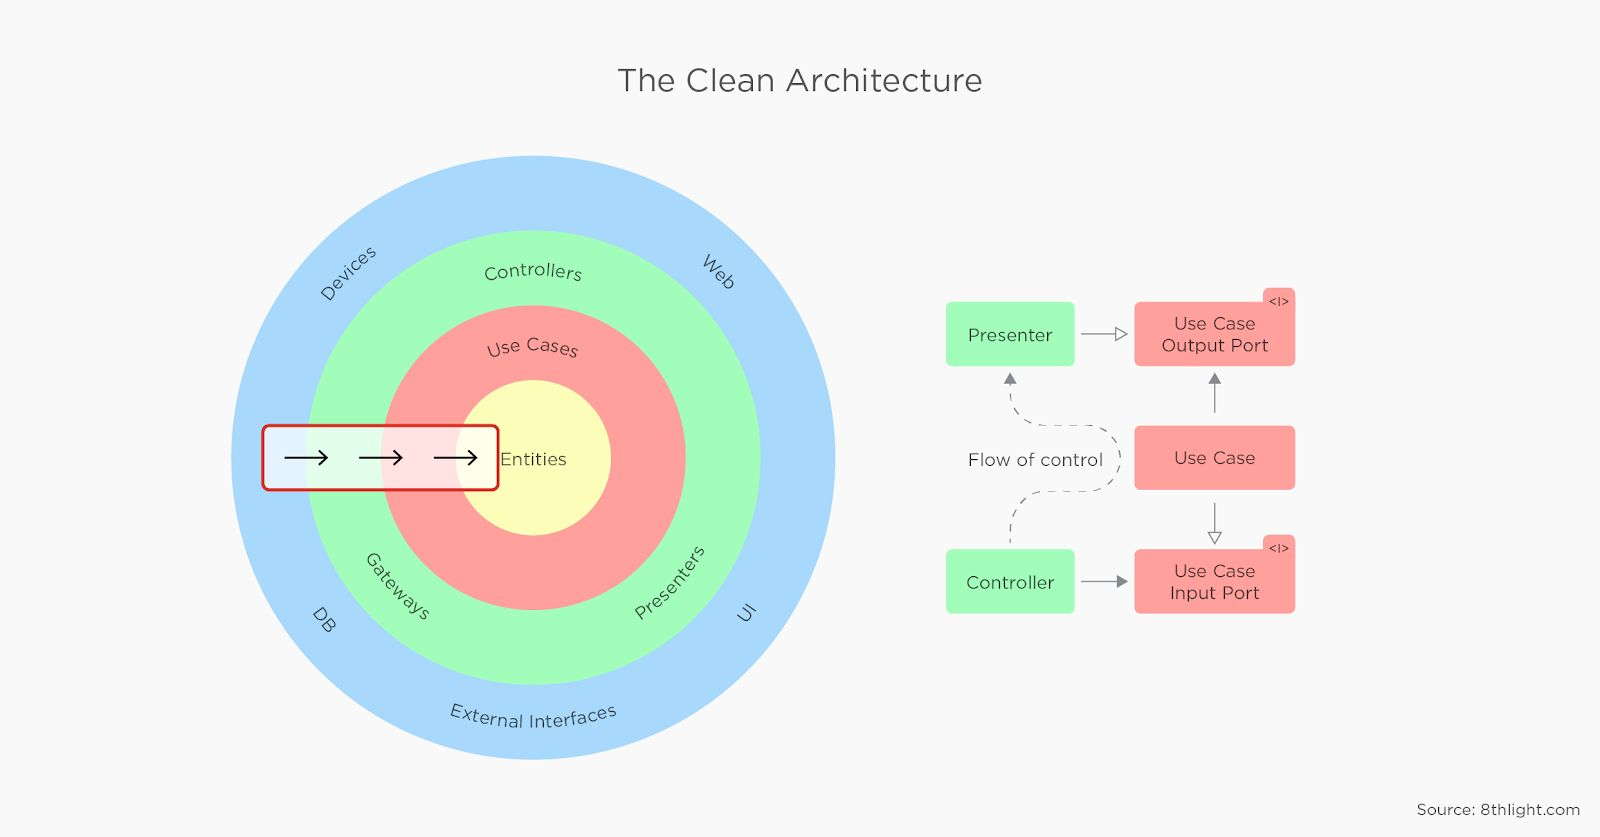
\includegraphics[width=1\textwidth]{Figures/-001.png}
	\rule{35em}{1pt}
	\caption[Principio de Dependecias]{Esquema de dependencias para una arquitectura en capas.}
	\label{fig:Diagrama_clasico}
\end{figure}


Las capas externas deben depender de las capas internas. Esas tres flechas en el cuadro rojo representan dependencias. En lugar de "depende", tal vez sea mejor usar términos como ''ve'', ''conoce'' o ''está consciente de...''. En estos términos, las capas externas ven, conocen y son conscientes de las capas internas, pero las capas internas no ven ni conocen, ni son conscientes de, las capas externas. Como dijimos anteriormente, las capas internas contienen lógica de negocios y las capas externas contienen detalles de implementación. Combinado con la regla de dependencia, se deduce que la lógica de negocio no ve, ni conoce, detalles de implementación. Y eso es exactamente lo que estamos tratando de lograr.

No existe una única forma de implementar esta regla dependerá del encargado del proyecto. Una estrategia consiste en colocar las clases de cada capa en paquetes diferentes, poniendo especial cuidado en no importar paquetes ''externos'' en paquetes ''internos''. Sin embargo, si algún programador del equipo no es consciente del principio de dependencias, nada les impediría romperlo. Un mejor enfoque sería separar las capas en diferentes módulos de Android, por ejemplo, y ajustar las dependencias en el archivo de construcción para que la capa interna simplemente no pueda utilizar la capa externa, sin embargo este enfoque implica un exaustivo conocimiento de la herramineta de construccion de la plataforma para la que se está desarrollando.

\subsection{Principio de Abstracción}
El principio de la abstracción ya se ha insinuado antes. Dice que, a medida que se están moviendo hacia el centro del diagrama, las cosas se vuelven más abstractas. Eso tiene sentido: como lo repetimos anteriormente el círculo interno contiene lógica de negocios y el círculo exterior contiene detalles de implementación.

\begin{figure}[htbp]
	\centering
	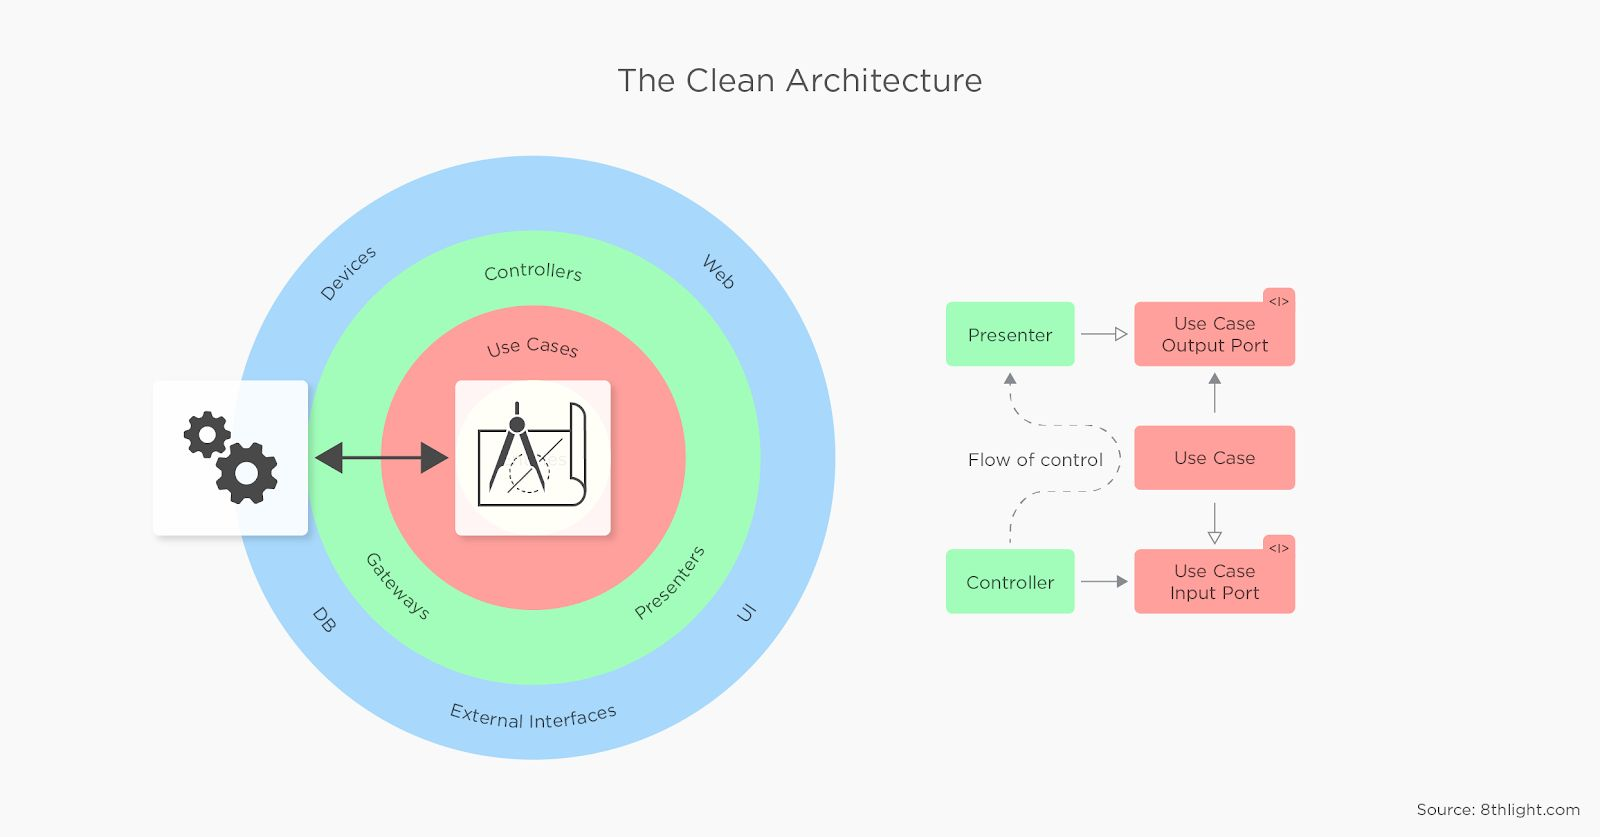
\includegraphics[width=1\textwidth]{Figures/-002.png}
	\rule{35em}{1pt}
	\caption[Abstraction Principle]{Principio de Abstracción en una arquitectura por capas.}
	\label{fig:C2_PA}
\end{figure}

Incluso puede plantearse el mismo componente lógico dividido entre varias capas, como se muestra en el diagrama. La parte más abstracta se puede definir en la capa interna, y la parte más concreta en la capa externa.

De esta manera, la lógica de negocios podría producir como un efecto secundario que se muestren notificaciones del sistema por ejemplo, pero no sabe nada acerca de los detalles de la implementación (cómo se implementan las notificaciones para una plataforma dada) . Además, la lógica empresarial ni siquiera sabe que existen detalles de implementación. Por lo tanto la regla de las dependencias se conserva.


\begin{figure}[htbp]
	\centering
	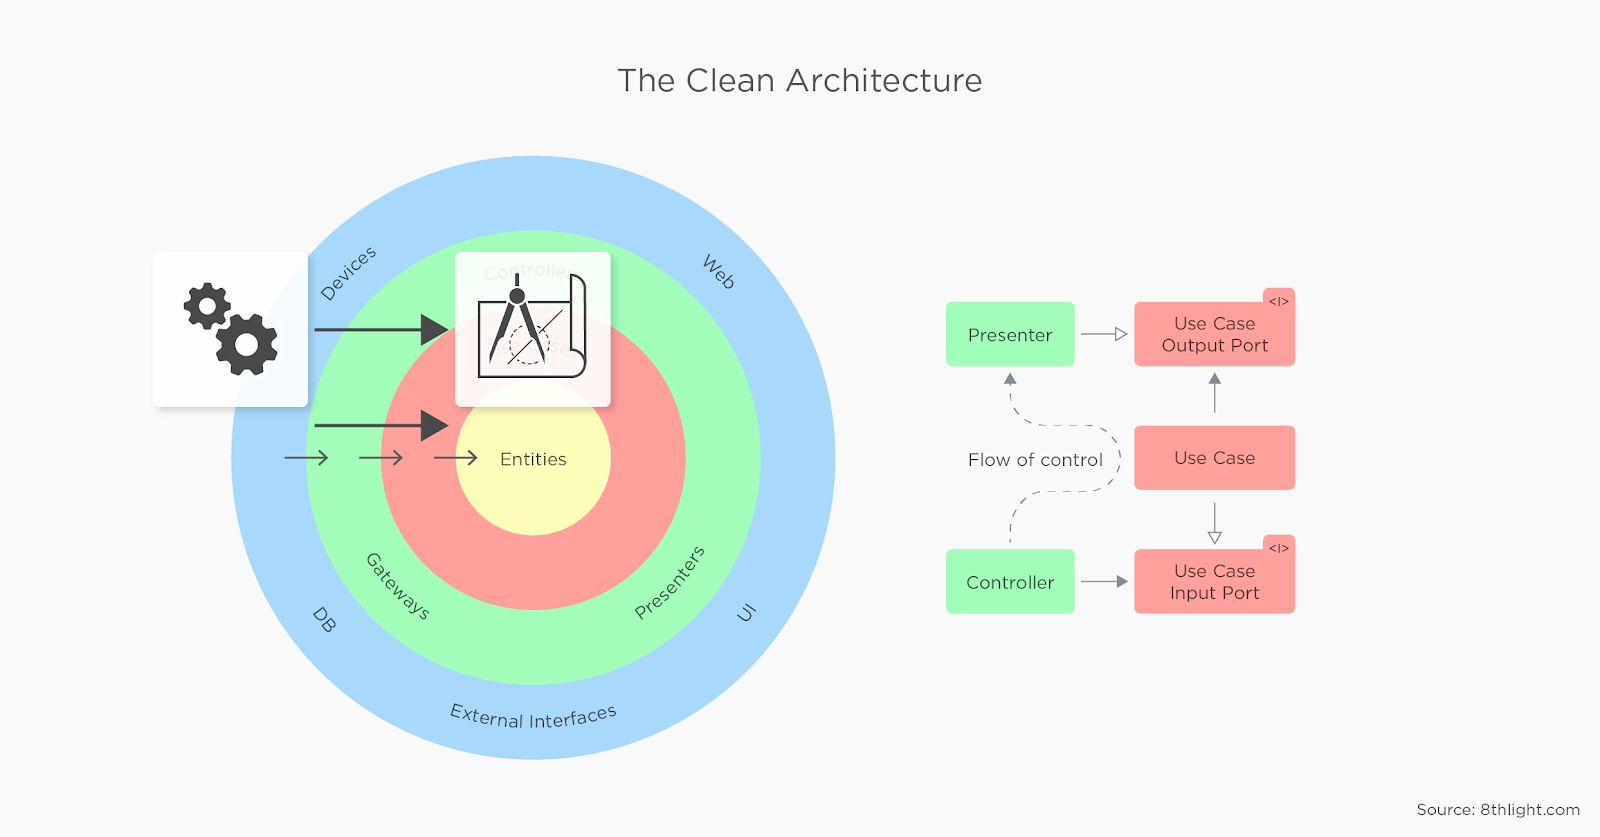
\includegraphics[width=1\textwidth]{Figures/-003.png}
	\rule{35em}{1pt}
	\caption[Abstraction Principle]{Principio de Abstracción en una arquitectura por capas.}
	\label{fig:C2_PA_02}
\end{figure}

\subsection{Comunicación entre Capas}
La lógica del negocio está en el medio y debe mediar entre los sitemas externos de salida y los sistemas externos de entrada como la interfaz de usuario, pero ni siquiera sabe que esos dos tipos existen. Esta es una cuestión de comunicación y flujo de datos. Necesitamos que los datos sean capaces de fluir de las capas externas a las internas y viceversa, pero la regla de dependencia no lo permite.

Sólo tenemos dos capas, la verde y la roja. El verde es exterior y sabe sobre el rojo, y el rojo es interior y sólo se conoce a sí mismo. Necesitamos que los datos fluyan desde el verde al rojo y viceversa. La solución ya se ha insinuado antes y se muestra en el siguiente diagrama:

\begin{figure}[htbp]
	\centering
	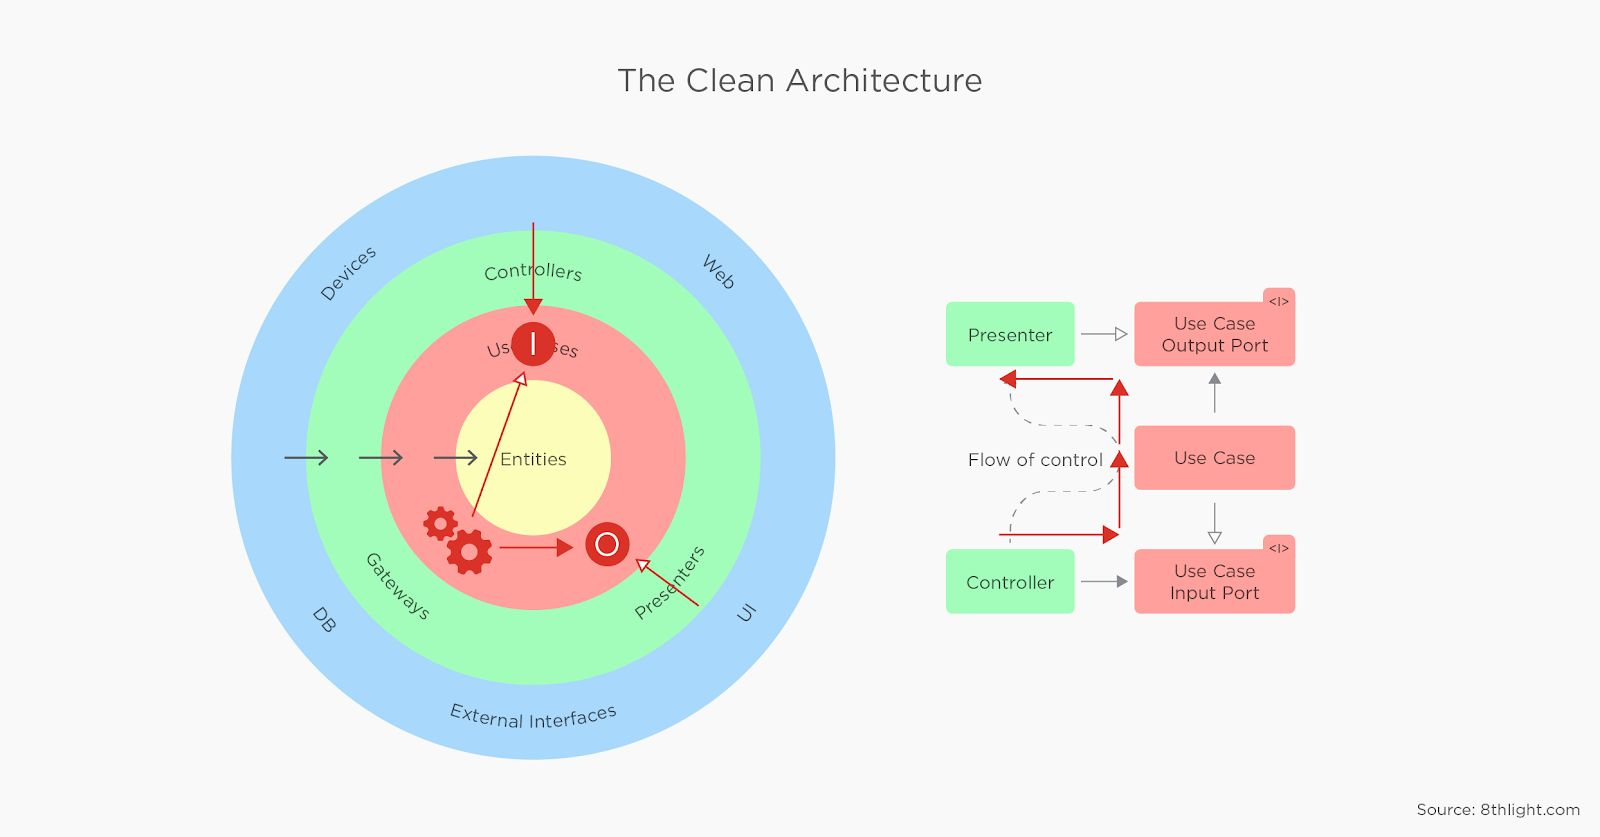
\includegraphics[width=1\textwidth]{Figures/-004.png}
	\rule{35em}{1pt}
	\caption[Layer Communication]{Comunicación entre capas.}
	\label{fig:C2_CC_01}
\end{figure}

La parte del diagrama en la parte inferior derecha muestra el flujo de datos. Los datos van desde el controlador, a través del puerto de entrada del caso de uso (o reemplazar el caso de uso con el componente de su elección), luego a través del propio caso de uso y después a través del puerto de salida del caso de uso al presentador.

El controlador tiene un puerto de entrada, literalmente tiene una referencia a él. Llama a un método en él, de modo que los datos van del controlador al puerto de entrada. Pero el puerto de entrada es una interfaz, y la implementación real es el caso de uso: por lo que ha llamado un método en un caso de uso y los flujos de datos al caso de uso. El caso de uso hace algo y quiere enviar los datos de vuelta. Tiene una referencia al puerto de salida, ya que el puerto de salida está definido en la misma capa, por lo que puede llamar al método en él. Por lo tanto, los datos van al puerto de salida. Y finalmente, el presentador es, o implementa, el puerto de salida.

\section{Arquitectura Hexagonal}
La arquitectura hexagonal comparte el enfoque de división de capas y utiliza los principios que la anterior sin embargo coloca a la DB en el centro del control del flujo de datos por lo que la diferencia real entre ambas es meramente de implementación y consideración.

\section{Arquitectura VIPER para iOS}
VIPER significa Views, Interactors, Presenters, Entities and Routing. La combinación de todos estos componentes vive dentro del llamado Módulo. La principal motivación detrás de esta arquitectura es proporcionar una solución a un problema en iOS conocido como Massive View Controllers. La arquitectura MVC tradicional utilizada para desarrollar la aplicación iOS simplemente no proporciona suficiente modularidad y separación de responsabilidades. Las partes View y Model permanecen más o menos limpias, pero toda la complejidad termina en ViewControllers, que tienen que manejar demasiadas cosas. Más de 1000 líneas de código no es poco común para un ViewController relativamente rico en funciones.

\begin{figure}[htbp]
	\centering
	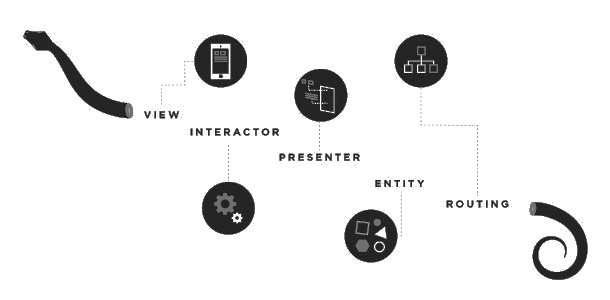
\includegraphics[width=1\textwidth]{Figures/-005_bw.png}
	\rule{35em}{1pt}
	\caption[VIPER Arch]{Esquema arquitectura VIPER.}
	\label{fig:C2S3_VA_01}
\end{figure}

Nuevamente se trata de una arquitectura separada por capas con separación de responsabilidades. En el caso de esta arquitectura en particular el único aspecto que cabe la pena hacer énfasis es en el esquema de comunicación que tiene lugar entre el Presentador y el Interactor. El Interactor trabaja con las Entidades y nunca las pasa al Presentador. En su lugar, los llamados objetos DisplayData se construyen a partir de las Entidades. Estos objetos contienen sólo los datos requeridos por el presentador que se mostrarán en la vista.

Hay un par de aspectos a los que uno debe prestar especial cuidado al utilizar la arquitectura VIPER en iOS. Lo primero es que uno tiene que instanciar todos los componentes con sus dependencias y hacer todo el cableado entre ellos en un módulo. Esto puede dar la impresión de que se está escribiendo demasiado del mismo código, cada vez que se crea un nuevo módulo, pero no hay forma de evitarlo. Es posible automatizar un poco este proceso escribiendo fragmentos de código personalizado y scripts de generación de código, pero muchas veces los resultados son demasiado generales para el módulo específico que estamos construyendo actualmente.

Otra aspecto difícil de manejar viene como resultado del cableado manual mencionado anteriormente - referencias cíclicas fuertes. Puesto que algunos de los componentes necesitan sus referencias cíclicas para trabajar, por ejemplo Presenter <-> Interactor, es posible generar memory leaks con gran facilidad si no se presta atención al momento de comunicar los objetos, cuáles referencias pueden ser fuertes y cuáles deben ser débiles. Esta tarea se vuelve más complicada cuanto más componentes y módulos hay en la aplicación. Es posible que se produzcan fugas adicionales de memoria ocultas cuando se usen características de lenguaje como los closures de Swift, así que uno debe ser muy cuidadoso al llamar a los métodos de Presenter desde un closure localizado dentro del Interactor.

Por último, esta estricta separación de las responsabilidades a veces conduce a tener Presenters muy simples, que sólo reorientar algunos flujos de datos de la Vista a los Interactores. Esto sucede cuando la arquitectura se aplica a unas pantallas relativamente simples, que no tienen muchas cosas que el Presentador pueda hacer.

\subsection{VIPER sobre Android}
\textit{La implementación de VIPER sobre android es impráctica y desbeneficiosa.}

Hay algunas diferencias significativas en la forma en que funcionan los SDK en iOS y Android. Android tiene Actividades, que son más o menos el equivalente de ViewControllers en iOS. Una gran diferencia es que uno no puede instanciar estos objetos. Uno puede pedirle al framework para iniciar una Actividad y luego puede anular sus métodos de ciclo de vida para hacer cualquier trabajo necesario. Por lo tanto, al implementar módulos VIPER, uno no puede realizar todo el cableado en una clase Wireframe cuando se instancia la actividad. En su lugar, todo el cableado del módulo VIPER inicial tiene que tener lugar cuando una Actividad es inicializada por el propio Framework. El SDK de Android también proporciona Fragmentos, que de hecho pueden ser instanciados por el programador, pero hay tanta magia relacionada con la creación de Fragmentos que el framework hace automáticamente, que hacen muy dificil controlar el ciclo de vida de tales Fragmentos. Por lo tanto, No considero el uso de Fragmentos como las vistas de VIPER e instanciándolas explícitamente en un Wireframe como una solución estable. Luchar contra el framework es siempre una mala idea.

Otra cosa específica en Android son los cambios de configuración, que normalmente destruyen toda la interfaz de usuario y la recrean. Eso incluye Actividades, Fragmentos y Vistas. Eso puede resultar catastrófico, porque todo el Módulo VIPER será eliminado por el recolector de basura (garbage colector) y recreado de nuevo. Así que uno tiene que asegurarse de que el estado de los componentes del módulo se guarda de alguna manera. Además, hay que tener cuidado con los objetos de larga vida y las operaciones de mantenimiento de las referencias a los componentes del módulo, ya que podría causar grandes fugas de memoria. Un ejemplo típico es una operación de petición de red, que tiene una referencia fuerte al Interactor del Módulo como su devolución de llamada. Dado que el Interactor tiene referencia al presentador y mantiene referencia a la vista, que contiene referencia a todas las cosas de la interfaz de usuario, esto podría dar lugar a una pérdida de memoria grande. Así que uno tiene que cuidar de limpiar tales referencias cuando un Módulo entero está siendo destruido y recreado.

Por estas razones se decidió descartar el uso de VIPER en el desarrollo de las apps como conseción y optar por implementar el enfoque de la Clean Architecture.


\newpage

 
%% Chapter Template

\chapter{Desarrollo} % Main chapter title

En el presente capítulo se describe el proceso de desarrollo del sistema que se compone en 3 partes, las cuales se detallan en cada caso el procedimiento de diseño e implementación utilizando como referencia el Documento de Especificación de Requerimientos de Sistema de \textit{Software} propuesto por la \textit{IEEE}.\\

\label{Chapter3} % Change X to a consecutive number; for referencing this chapter elsewhere, use \ref{ChapterX}

\lhead{Capítulo 3. \emph{Desarrollo}} % Change X to a consecutive number; this is for the header on each page - perhaps a shortened title

%----------------------------------------------------------------------------------------
%	SECTION 1
%----------------------------------------------------------------------------------------
\section{Análisis del problema}
El problema consiste en comunicar a través de Internet, notificaciones de alertas producidas por un dispositivo que contiene sensores, hacia un servidor remoto el cual recibe y almacena dichas notificaciones y, eventualmente puede tomar decisiones acerca de las mismas a través de un operador que monitoriza el sistema. \\
Por otro lado, el control del dispositivo se debe realizar a través de un teléfono móvil inteligente(\textit{smartphone}) a través de la red LAN del hogar. Éste, a su vez, puede ser conectado con otros aparatos eléctricos para comandarlos en caso de ser necesario.\\
Por lo tanto, se decidió dividir el problema en 3 partes, las cuales fueron diseñadas para poder ser desarrolladas concurrentemente. Éstas son: Un subsistema encargado de la monitorización de los sensores(alarma), otro que recibe las notificaciones y emite alertas(Servidor) y por último, el encargado de comunicar al usuario con la alarma (aplicación).
\newpage

%% Chapter Template

\chapter{Descripción del modelo experimental} % Main chapter title

\label{Chapter4} % Change X to a consecutive number; for referencing this chapter elsewhere, use \ref{ChapterX}

\lhead{Capítulo  4. \emph{Descripción del modelo experimental}} % Change X to a consecutive number; this is for the header on each page - perhaps a shortened title

Se definieron 3 modelos experimentales, donde los niveles de abstracción fueron disminuyendo hasta el último, donde se realizaron las pruebas en condiciones reales.\\
El primer modelo, el virtual, representa el sistema en su totalidad en un entorno local, simulando los subsistemas a través de módulos de software.\\
El siguiente fué el modelo físico, donde en cada subsistema se utilizó sobre la arquitectura de \textit{hardware} correspondiente, pero en un entorno de red local.\\
Una vez comprobado que el sistema actuó correctamente en un ambiente físico real aunque limitado, se continuó con el último modelo que fué el real. En este caso, cada sistema se ejecutó en su ambiente real sin limitaciones de conectividad y con la totalidad de sus funcionalidades.\\
En las siguientes secciones se detallan las características de cada modelo.


\newpage


%----------------------------------------------------------------------------------------
%	SECTION 1
%----------------------------------------------------------------------------------------

\section{Modelo virtual}

Como se muestra en la figura \ref{Diagrama_virtual}, este modelo consiste  en probar los subsistemas a través de módulos de \textit{software} ejecutados en la misma computadora, que simulaban el sistema real:\\

\begin{figure}[htbp]
	\centering
		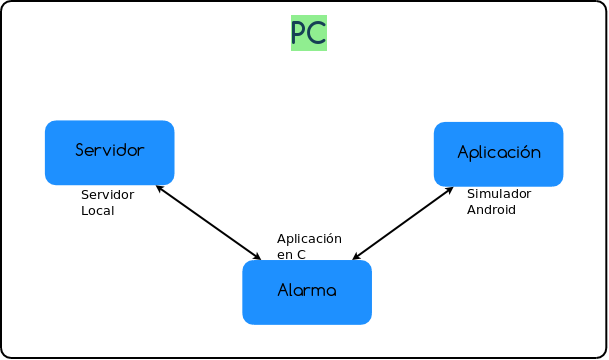
\includegraphics[width=0.8\textwidth]{Figures/Diagrama_virtual.png}
		\rule{35em}{1.5pt}
	\caption[Modelo Virtual del sistema]{Modelo Virtual del sistema}
\label{Diagrama_virtual}
\end{figure}

\begin{figure}[htbp]
	\centering
		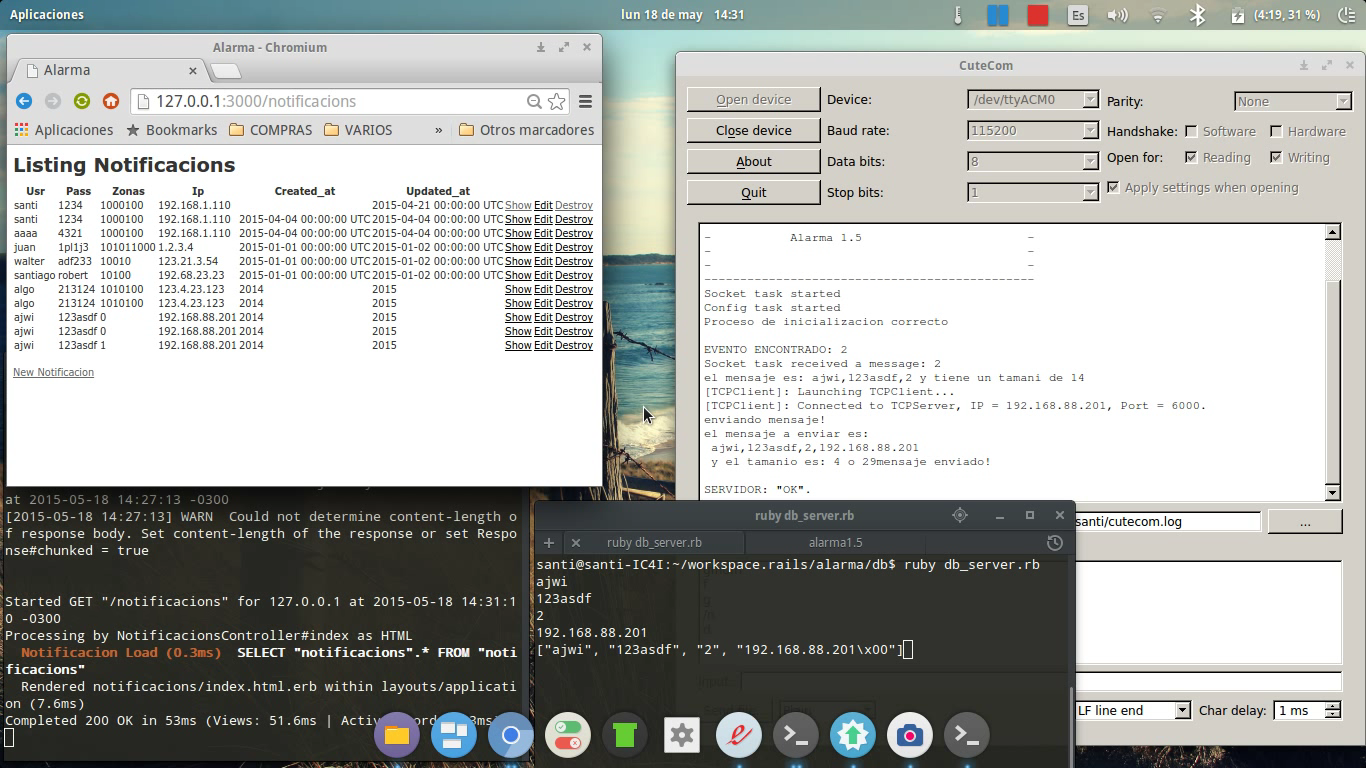
\includegraphics[width=1\textwidth]{Figures/captura_virtual.png}
		\rule{35em}{1.5pt}
	\caption[Captura de pantalla de modelo virtual del sistema]{Captura de pantalla de modelo virtual del sistema}

\end{figure}

A continuación se detalla las funcionalidades básicas propias y de comunicación con el resto de los subsistemas, indicando también, sus limitaciones en cada caso.

\newpage


%-----------------------------------
%	SUBSECTION 1.1
%-----------------------------------
	\subsection{Módulo Alarma}

En el caso de la alarma, se desarrolló un programa en C, que simula las alertas y envía notificaciones al servidor.\\
Limitaciones:
\begin{itemize}
\item Recibe órdenes (activar/desactivar) que simplemente limitan al envío de las notificaciones.
\item No se provee autenticación ni cuenta con salidas para comandar.
\end{itemize}


%-----------------------------------
%	SUBSECTION 1.2
%-----------------------------------

	\subsection{Módulo Servidor}

El servidor, realizado en Ruby sobre el \textit{framework Rails}, integra un \textit{script} que recibe notificaciones por \textit{socket} desde la alarma y las muestra en un servidor \textit{web}.\\
Limitaciones:
\begin{itemize}
\item La interfaz gráfica se limita la exposición de las notificaciones en texto plano.
\item El modelo de la base de datos contempla una única tabla donde se resguardan todos los datos.
\item El controlador del servidor WEB no permite realizar CRUD sobre los datos de los usuarios.
\end{itemize}

%-----------------------------------
%	SUBSECTION 1.3
%-----------------------------------

	\subsection{Módulo Aplicación}

Consta de un \textit{software} hecho en Java sobre el \textit{IDE Android Studio}, que envía ordenes por socket a la alarma y recibe las respuestas de la misma.\\
Limitaciones:
\begin{itemize}
\item Este programa se ejecuta sobre un emulador de teléfonos Android.
\item No permite autenticación.
\end{itemize}

\newpage

%----------------------------------------------------------------------------------------
%	SECTION 2
%----------------------------------------------------------------------------------------

\section{Modelo físico}

Una vez comprobada la funcionalidad en el ambiente virtual, se pasó a un ambiente físico controlado y limitado.
El mismo se representa en la figura \ref{Diagrama_fisico}:

\begin{figure}[htbp]
	\centering
		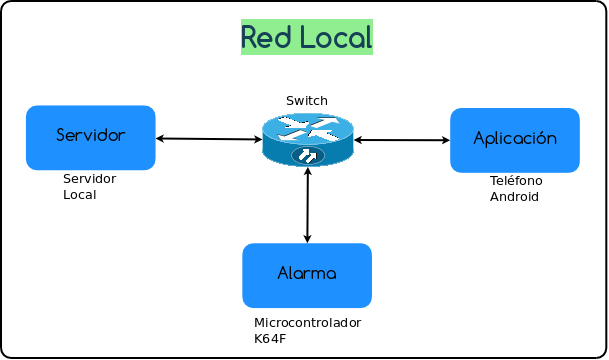
\includegraphics[width=0.8\textwidth]{Figures/Diagrama_fisico.png}
		\rule{35em}{1.5pt}
	\caption[Modelo Físico del sistema]{Modelo Físico del sistema}
\label{Diagrama_fisico}
\end{figure}

Se puede ver que la ejecución del sistema, si bien es sobre la arquitectura correspondiente, la conectividad es limitada a un ambiente de red local y las funcionalidades de cada subsistema no contemplan aún la totalidad de los requerimientos, aunque si los básicos y algunos secundarios.
\newpage


%-----------------------------------
%	SUBSECTION 2.1
%-----------------------------------
	\subsection{Módulo Alarma}

Se desarrolló sobre el microcontrolador K64F, utilizando el \textit{IDE KDS} y el SO \textit{MQX}. \\
Limitaciones:
\begin{itemize}
\item En el caso de los sensores, solo se limitan a interruptores que accionan las alertas, que luego se transmiten en la red local hasta el servidor. 
\item Las notificaciones se restringen a la red local.
\end{itemize}

%-----------------------------------
%	SUBSECTION 2.2
%-----------------------------------

	\subsection{Módulo Servidor}

El servidor se mantuvo en una computadora local, se agregaron funcionalidades \textit{CMS} al servidor \textit{web} para administrar las alarmas y autenticación en las notificaciones entrantes. \\

Limitaciones:
\begin{itemize}
\item Las actualizaciones en la vista del servidor no se realizan automáticamente.
\item Acceso únicamente en red local.
\end{itemize}
\newpage

%-----------------------------------
%	SUBSECTION 2.3
%-----------------------------------

	\subsection{Módulo Aplicación}

Se añadieron múltiples comandos, que se ejecutan directamente desde el teléfono conectado vía \textit{WiFi} a la red local, hacia la alarma. También se mejoró la interfaz de usuario, como se puede ver en la figura \ref{app}:\\

\begin{figure}[htbp]
	\centering
		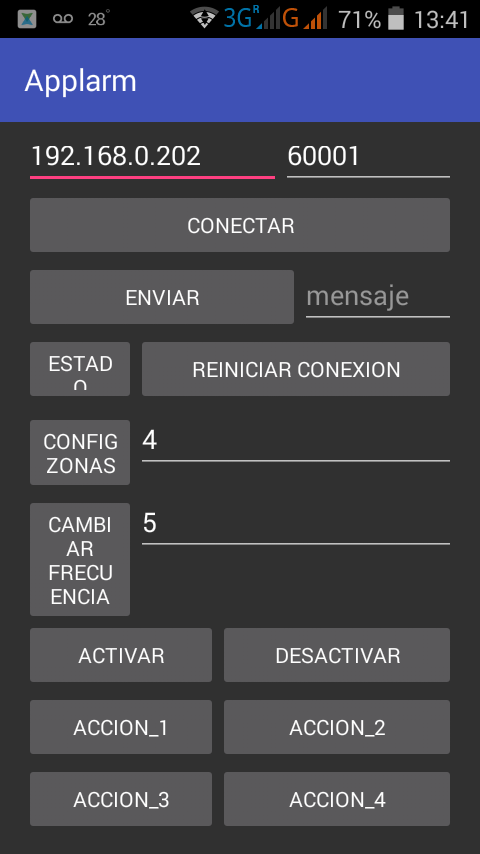
\includegraphics[width=0.5\textwidth]{Figures/app.png}
		\rule{35em}{1.5pt}
	\caption[Captura de App]{Captura de App}
\label{app}
\end{figure}
\newpage

%----------------------------------------------------------------------------------------
%	SECTION 3
%----------------------------------------------------------------------------------------

\section{Modelo real}

En esta etapa, una vez superadas las pruebas en un entorno restringido, se dio comienzo a las pruebas de campo con el prototipo real.\\
Se añadieron algunas mejoras en las interfaces gráficas y nuevas funcionalidades secundarias, detalladas posteriormente.
El esquema se representa a continuación en la figura \ref{Diagrama_real}:\\	

\begin{figure}[htbp]
	\centering
		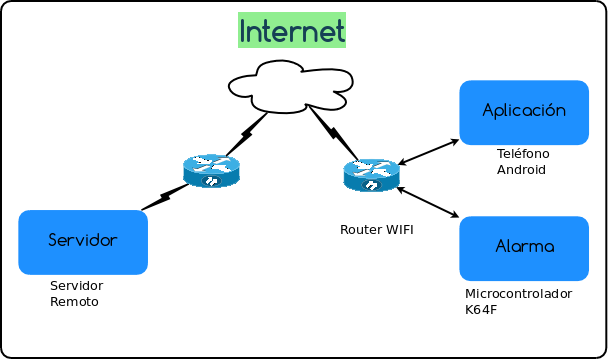
\includegraphics[width=0.8\textwidth]{Figures/Diagrama_real.png}
		\rule{35em}{1.5pt}
	\caption[Modelo Real del sistema]{Modelo Real del sistema}
\label{Diagrama_real}
\end{figure}

\newpage


%-----------------------------------
%	SUBSECTION 3.1
%-----------------------------------
\subsection{Módulo Alarma}

Se agregó la capacidad de comandar elementos externos, a través de un \textit{shield} desarrollado para el microcontrolador.\\
Se añadieron los sensores correspondientes para detectar las alertas.
La figura \ref{pcb} y \ref{relay_shield}, detalla se composición:\\
\begin{figure}[htbp]
	\centering
		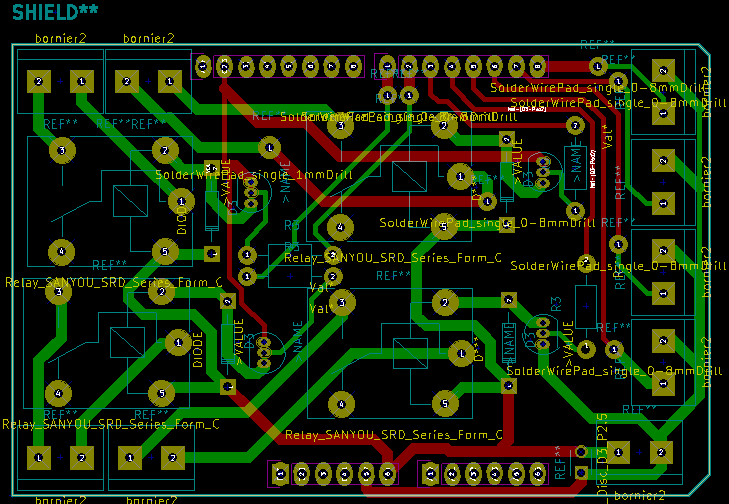
\includegraphics[width=0.8\textwidth]{Figures/pcb.png}
		\rule{35em}{1.5pt}
	\caption[PCB]{PCB}
\label{pcb}
\end{figure}

\begin{figure}[htbp]
	\centering
		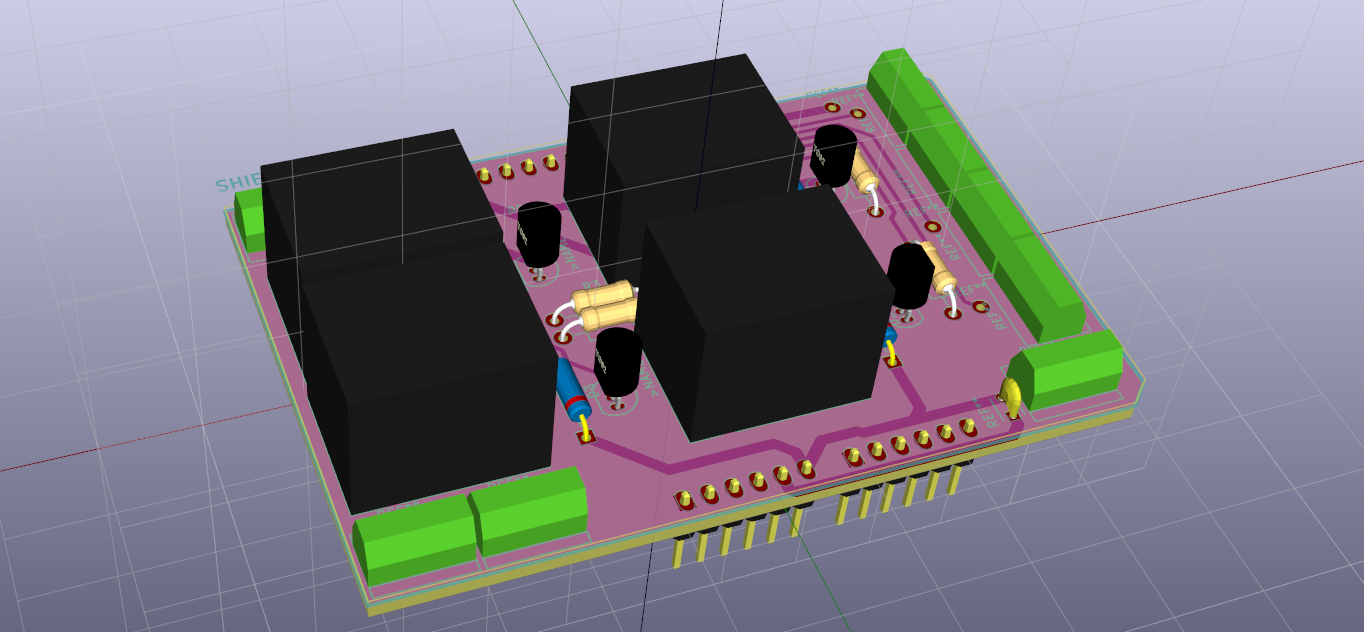
\includegraphics[width=1\textwidth]{Figures/relay_shield.png}
		\rule{35em}{1.5pt}
	\caption[Vista 3D \textit{shield}]{Vista 3D \textit{shield}}
\label{relay_shield}
\end{figure}
\newpage

%-----------------------------------
%	SUBSECTION 3.2
%-----------------------------------

\subsection{Módulo Servidor}

Se montó el servidor, en una \textit{PC} dedicada para tal fin. Para dotarla de acceso remoto se \textit{forwardearon} los puertos del \textit{router} necesarios para que redirigiera las conexiones hacia el servidor.\\
Por otro lado, se utilizó un servicio de \textit{DDNS}, para mantener un dominio fijo y que el servidor pueda ser encontrado ante un cambio de IP (ya que no se contaba con una dirección IP estática pública).\\
Se añadieron notificaciones automáticas vía \textit{E-mail} a los usuarios de las alarma.\\
Por último, se mejoró el \textit{frontend} como se puede apreciar en la figura \ref{servidor}, con la ayuda de \textit{JavaScript} y se agregó autenticación de usuario para el administrador del sistema. Además se utilizó el \textit{framework Bootstrap} para añadir una mejora gráfica en la interfaz de usuario hecha en HTML5. \\

\begin{figure}[htbp]
	\centering
		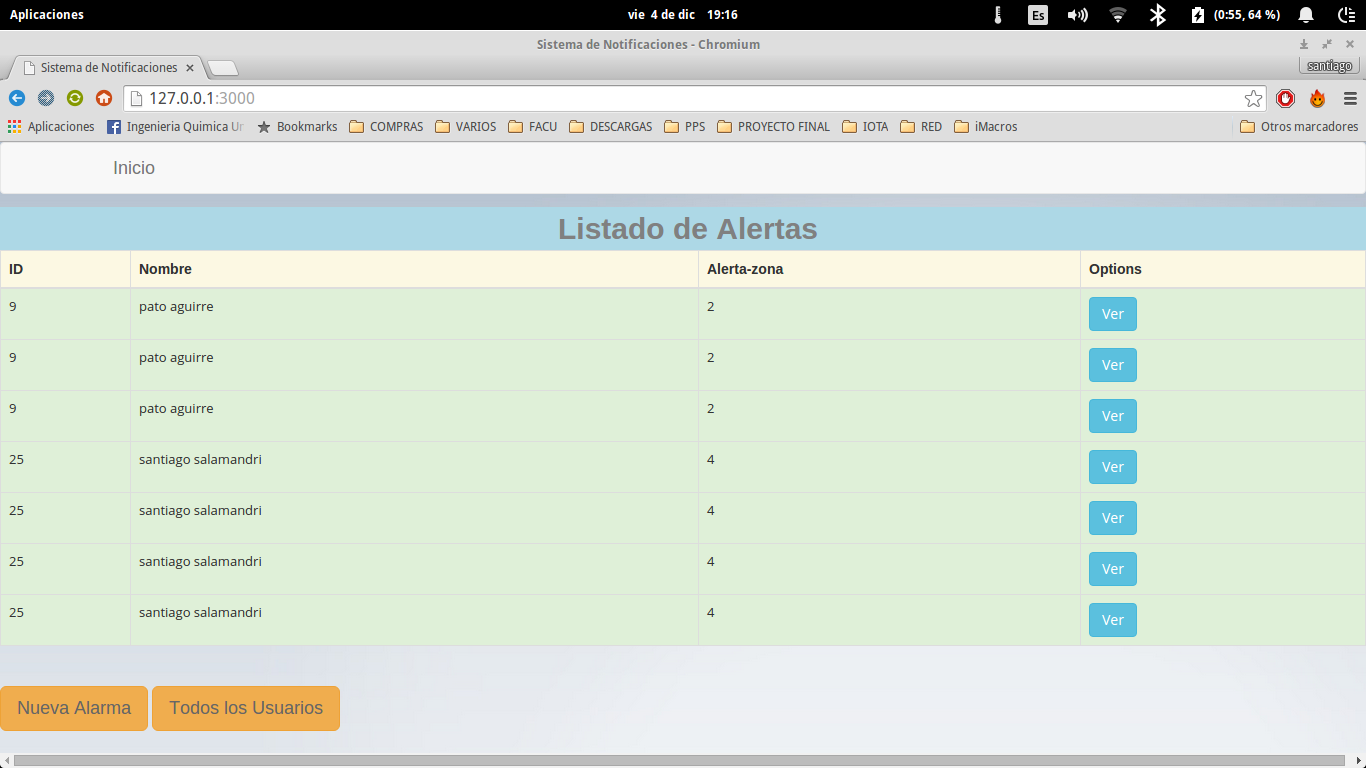
\includegraphics[width=1\textwidth]{Figures/servidor.png}
		\rule{35em}{1.5pt}
	\caption[Servidor]{Servidor}
\label{servidor}
\end{figure}
\newpage

%-----------------------------------
%	SUBSECTION 3.2
%-----------------------------------

\subsection{Módulo Aplicación}

Se mejoró la interfaz gráfica, removiendo botones innecesarios y separando las actividades de configuración de las de comando remoto. En la figura \ref{app_final}, se exhiben los cambios realizados:\\

\begin{figure}[htbp]
	\centering
		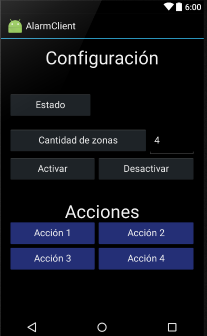
\includegraphics[width=0.5\textwidth]{Figures/app_final.png}
		\rule{35em}{1.5pt}
	\caption[Captura de App final]{App Final}
\label{app_final}
\end{figure}
\newpage 
% Chapter Template

\chapter{Clean Architecture} % Main chapter title

\label{Chapter5} % Change X to a consecutive number; for referencing this chapter elsewhere, use \ref{ChapterX}

\lhead{Capítulo  5. \emph{Clean Architecture}} % Change X to a consecutive number; this is for the header on each page - perhaps a shortened title

%----------------------------------------------------------------------------------------
%	SECTION 1
%----------------------------------------------------------------------------------------

\section{Modelos de Implementación Clean Architecture}

Los mejores intentos de implementación de esta arquitectura vienen de la mano de un colega Fernando Cejas y el ejemplo de los Blueprints de Google.

\begin{figure}[htbp]
	\centering
	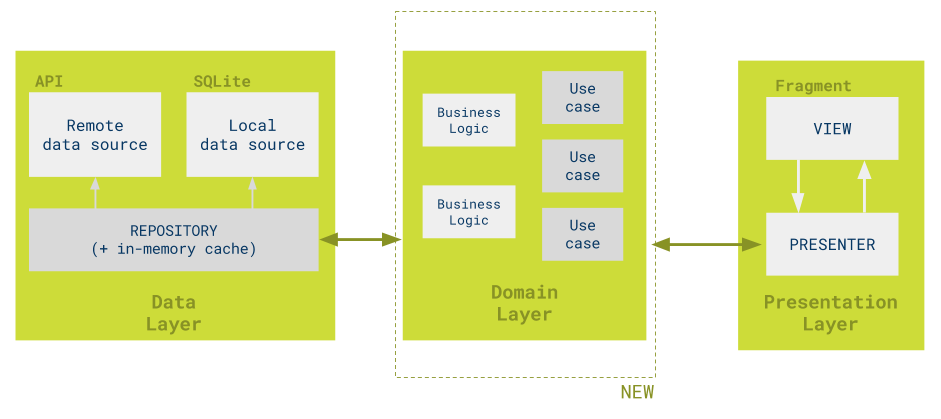
\includegraphics[width=1\textwidth]{Figures/-006.png}
	\rule{35em}{1pt}
	\caption[Principio de Dependecias]{Esquema de dependencias para una arquitectura en capas.}
	\label{fig:Diagrama_clasico}
\end{figure}

Ambas implementaciones están compuestas de tres capas distintas:

\begin{itemize}
	\item Presentation Layer: Esta capa se encarga de interactuar con la UI. Implementa un patrón de diseño conocido como \textbf{MVP (Model View Controller)}. 
	\item Domain Layer: Esta capa contiene toda la lógica de negocio. La capa de dominio comienza con las clases denominadas casos de uso o interactores según la literatura, utilizados por los presentadores de la aplicación. Estos casos de uso representan todas las acciones posibles que un desarrollador puede realizar desde la capa de presentación. Los casos de uso se implementaron utilizando el patrón de diseño conocido como \textbf{Commander}.
	\item Data Layer: Esta capa administra la adquisición de datos y es capaz de utilizar diferentes fuentes de datos. Esta capa se suele implementar utilizando el patrón de diseño conocido como \textbf{Repository}.  
\end{itemize}

\section{Presentation Layer: MVP}
El patrón de arquitectura que se utiliza en la capa de presentación de ambas implementaciones se conoce como Modelo-Vista-Presentador.
La idea detrás del patrón es concentrar la lógica de la interacción con el usuario en una entidad conocida como presentador, las operaciones directamente relacionadas con la manipulación de objetos gráficos y la captura de acciones de usuario están delegadas a la entidad Vista, finalmente la adquisición de datos y la ejecución de los algoritmos que encapsulan la lógica de negocio forman parte de las entidades modelo en el patrón.
El diagrama de componentes que describe la relación entre las partes principales se puede observar a continuación

\begin{figure}[htbp]
	\centering
	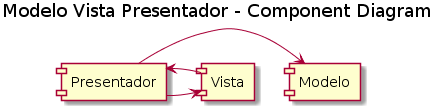
\includegraphics[width=0.7\textwidth]{Figures/uml_mvp_component.png}
	\rule{35em}{1pt}
	\caption[MVP Components]{Diagrama de componentes del patrón.}
	\label{fig:uml_mvp_component}
\end{figure}

Es posible deducir el esquema de comunicación entre los componentes a partir del diagrama. La vista se comunica de manera bidireccional con el presentador y cuando es necesario el presentador se comunica de manera unidireccional con el modelo.

\begin{figure}[htbp]
	\centering
	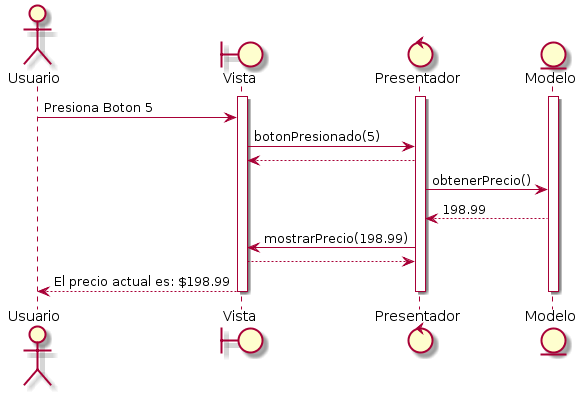
\includegraphics[width=0.7\textwidth]{Figures/uml_mvp_sequence.png}
	\rule{35em}{1pt}
	\caption[MVP Sequence]{Diagrama de secuencia para una interacción con el usuario.}
	\label{fig:uml_mvp_sequence}
\end{figure}

Una convención para la implementación del patrón es tratar de generar vistas completamente ajenas de cualquier lógica operativa y agnósticas del estado de la aplicación. Esto las convierte en un mero instrumento de interfaz entre lo que percibe el usuario y sus reacciones. 

Otra de las convenciones sugiere utilizar objetos modelo-vista en la comunicación entre el presentador y la vista para estandarizar el tipo de mensaje y el proceso de actualización de la vista.

En el caso de las implementaciones antes mencionadas la interface con el modelo es satisfecha mediante el uso de objetos casos de uso ó interactores, ambos términos siuelen utilizarse de manera intercambiable.

\section{Domain Layer: Commander Pattern}
El patrón de diseño conocido como Commander se utiliza para abstraer la ejecución de procedimientos mediante la implementación de entidades comando. Estos objetos ejecutan un único algoritmo y para ello establecen dos entidades adicionales: 
\Agregar diagrama de clases, secuencia original, secuecnia modificado por arquitectura y mapeo de entidades con entidades de arq
\begin{itemize}
	\item Solicitud (Request): Un objeto que contiene el conjunto de parametros de entrada que deben ser satisfechos para poder realizar la ejecución de la rutina del comando.
	\item Respuesta (Response): Un objeto que contiene los valores que se obtuvieron de la ejecución del algoritmo del comando.
\end{itemize}

Por lo tanto puede inferirse el flujo de operación y ejecución de los comandos.

\begin{enumerate}
\item La entidad ejecutora crea una instancia de un comando 
\item La entidad ejecutora inicializa un objeto solicitud
\item La entidad ejecutora ejecuta el comando llamando al método ''ejecutar'' de dicho comando pasando como parámetro la solicitud previamente creada.
\item La unidad ejecutora observa los resultados en espera activa implementando el patrón Observer o mediante algún esquema de callback.
\end{enumerate}

\begin{figure}[htbp]
	\centering
	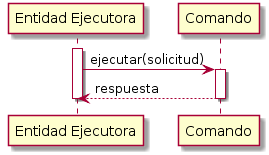
\includegraphics[width=0.5\textwidth]{Figures/uml_commander_sequence.png}
	\rule{35em}{1pt}
	\caption[MVP Components]{Diagrama de secuencia para el patrón Commander.}
	\label{fig:uml_commander_sequence}
\end{figure}

Siguiendo los lineamientos de la arquitectura propuesta los autores denominan a los comandos: Casos de Uso, ó Interactores.

Como una nota relevante de implementación se recomienda ejecutar las rutinas de los comandos en un hilo/proceso separado para para evitar bloquear el proceso principal de la apliación.

\section{Data Layer: Repository Pattern}
En la capa de datos se propone la implenentación de un patrón de diseño conocido como Repository(Repositorio). Este diseño intenta encapsular todas los orígenes de datos en una única interface. Para ello se define un objeto Repositorio que implementa la interfaz de orígen de datos. Así mismo otros objetos conocidos como Orígenes implementan la misma interfaz pero acceden distintas fuentes. La responsabilidad del Repositorio es determinar cual de esos orígen debe utilizarse para obtener los resultados para una determinada consulta de datos.
Por lo tanto la entidad que realiza la consulta de datos sólo debe conocer un sólo contrato, aquél de los Orígenes.
% 
 
%% Chapter Template

\chapter{Conclusiones} % Main chapter title

\label{Chapter6} % Change X to a consecutive number; for referencing this chapter elsewhere, use \ref{ChapterX}

\lhead{Chapter 6. \emph{Conclusiones}} % Change X to a consecutive number; this is for the header on each page - perhaps a shortened title

%----------------------------------------------------------------------------------------
%	SECTION 1
%----------------------------------------------------------------------------------------
Durante el desarrollo de la presente práctica se entendió las ventajas de implementar un sistema de software utilizando un patrón de arquitectura. La inspección de código escrito por profesionales del área introdujo conceptos de programación Java acanzados tales como el uso de clases anónimas y la implementación de clases y métodos genericos. Se pudo observar las teécnicas empleadas para realizar las pruebas sobre el código implementado y fue necesario invertir tiempo en la investigacion de las librerias y framework para pruebas tales como Mockito y Espress.\\
De manera indirecta se pudo observar cómo la definición de una arquitectura de estas caracterísitcas no solo tiene impacto en la organización y testabilidad del código sino también introduce un procedimeinto de trabajo tanto para la adición de nuevas funcionalides sino para la remoción de errores y la insepcción del código en general.\\
Como una desventaja notoria se menciona la empinada curva de aprendizaje para la inlcusión de nuevos miembros en un hipotético equipo de desarrollo. Así mismo se hizo evidente que todos los conceptos de abstracción que fueron introducidos se traducen en un aumento notable en la cantidad de lineas de código meramente dedicadas a mantener la estructura del diseño pero que no proveen una funcionalidad concreta al sistema.\\
Finalmente, se observaron inconsistencias entre el planteo teórico de la arquitectura y la implementación real del software mayormente por la dificultad técnica y conseciones en la que incurrieron los programadores para disminuir la verbosidad de algunos componentes o interacciones.
 
%----------------------------------------------------------------------------------------
%	THESIS CONTENT - APPENDICES
%----------------------------------------------------------------------------------------

\addtocontents{toc}{\vspace{2em}} % Add a gap in the Contents, for aesthetics

\appendix % Cue to tell LaTeX that the following 'chapters' are Appendices

% Include the appendices of the thesis as separate files from the Appendices folder
% Uncomment the lines as you write the Appendices

%% Appendix A

\chapter{Código} % Main appendix title

\label{AppendixA} % For referencing this appendix elsewhere, use \ref{AppendixA}

\lhead{Apéndice A1. \emph{Alarma}} % This is for the header on each page - perhaps a shortened title
\section{{\emph{Alarma}}}
Para ver el código implementado en la alarma, ingresar en el siguiente link:

\href{url}{https://bitbucket.org/santiagosalamandri/alarma\_1.5}

\subsection{Referencias utilizadas}
\begin{itemize}
\item Código:
	\begin{itemize}
	\item MQX RTOS\cite{embedded1}.
	\end{itemize} 
\item Diseño: 
	\begin{itemize}
	\item Diseño de alarma hogareña \cite{alarm1}.
	\item Como diseñar alarma \cite{alarm2}.
	\item Alarma hogareña Inalambrica\cite{alarm3}.
	\end{itemize}
	
\item Comunicación:
	\begin{itemize}
	\item TCP/IP Protocol Design \cite{socket1}.
	\item Socket\cite{socket9}.
	\end{itemize}
\item Circuito impreso:
	\begin{itemize}
	\item Kicad design\cite{pcb1}.
	\end{itemize}
\end{itemize}

\lhead{Apéndice A2. \emph{Servidor}} % This is for the header on each page - perhaps a shortened title
\section{{\emph{Servidor}}}
Para ver el código implementado en la servidor, ingresar en el siguiente link:

\href{url}{https://bitbucket.org/santiagosalamandri/web\_server3}
\subsection{Referencias utilizadas}
\begin{itemize}
\item Código:
\begin{itemize}
\item Desarrollo ágil Web \cite{rails1Book}.
\item Rails \cite{rails2Book}.
\item Ruby\cite{ruby1Book}.
\item Rails y Bootstrap\cite{rails1}.
\item JavaScript en Rails\cite{rails2}.
\item Módulo \textit{e-mail} \cite{rails3}.
\end{itemize}
		
\item Comunicación:
\begin{itemize}
\item BSD Sockets en Ruby\cite{socket2}.
\item Programación de Sockets en Ruby  \cite{socket3}.
\item Ruby Sockets \cite{socket4}.
\item Programación de Sockets\cite{socket5}.
\item Documentación de sockets en Ruby\cite{socket10}.
\end{itemize}
\item Base de datos:
	\begin{itemize}
	\item Queries SQL en Ruby\cite{sql1}
	\end{itemize}
\item \textit{Front-end}:
	\begin{itemize}
	\item Libro de Ajax\cite{ajax1Book}.
	\item Ajax en Ruby \cite{ajax1}.
	\item Tutorial de Ajax en Ruby \cite{ajax2}.
	\item Ajax y Boostrap \cite{ajax3}.
	\end{itemize}
\end{itemize}


\lhead{Apéndice A3. \emph{Aplicación}} % This is for the header on each page - perhaps a shortened title
\section{{\emph{Aplicación}}}

Para ver el código implementado en la aplicación, ingresar en el siguiente link:

\href{url}{https://bitbucket.org/santiagosalamandri/app-alarma-final}

\subsection{Referencias utilizadas}
\begin{itemize}
\item Código:
\begin{itemize}
\item Libro Desarrollo en Android\cite{android1Book}.
\item Tutorial Android \cite{android1}.
\item Tutorial Android Studio \cite{android2}.
\item Curso Programación Android \cite{android3}.
\end{itemize}

\item Comunicación:
\begin{itemize}
\item Ejemplos de Android Socket\cite{socket6}.
\item Tutorial de Android TCP conections \cite{socket7}.
\item Sockets en Android \cite{socket8}. 
\end{itemize}

\end{itemize}

\section{{\emph{PCB}}}
Para ver el proyecto del \textit{PCB} de la alarma, ingresar en el siguiente link:

\href{url}{https://bitbucket.org/santiagosalamandri/relay\_shield}


\addtocontents{toc}{\vspace{2em}} % Add a gap in the Contents, for aesthetics

\backmatter

%% Chapter Template
\bibliographystyle{unsrtnat} % Use the "unsrtnat" BibTeX style for formatting the Bibliography

\chapter{Bibliografía} % Main chapter title

%\label{Bibliografia} % Change X to a consecutive number; for referencing this chapter elsewhere, use \ref{ChapterX}
%\section{Bibliografía}

\lhead{\emph{Bibliografía}} % Change X to a consecutive number; this is for the header on each page - perhaps a shortened title

\begin{itemize}
\item A Software Testing Primer: An Introduction to Software Testing.Jenkins, Nick.Año 2008.
\item Applying Agile Methods to Embedded Systems Development,Doug Dahlby,PhD,Applying Agile Methods to Embedded Systems Development,Año 2004.\\
	\href{url}{http://embuild.org/dahlby/agileEm/agileEm.pdf} \\
	Última fecha de consulta: 07/03/2016.
\item Andrés Djordjalian,Desarrollo Ágil y Modelado,Año 2010.\\
	\href{url}{http://www.indicart.com.ar/~sase/Desarrollo\%20Agil\%20y\%20Modelado.pdf}\\
	Última fecha de consulta: 	 07/03/2016.
\item IEEE Recommended Practice for Software Requirements Specifications,IEEE Computer Society,Año 1998.\\
	\href{url}{http://www.cse.msu.edu/~cse870/IEEEXplore-SRS-template.pdf}\\
	Última fecha de consulta: 	 07/03/2016.
\item Software Engineering for Students, 4ta edición,Douglas Bell,Addison-Wesley,ISBN:978-0-32126-127-4,Año 2005.
\item Agile Web Development with Rails,4ta edición,Sam Ruby,Dave Thomas,David Heinemeier Hansson,The Pragmatic Programmers LLC,2010.
\item Head First Rails,David Griffiths,O'reilly,ISBN:978-0-596-51577-5,Año 2009.
\item Sockets programming in Ruby,M. Tim Jones,Año 2005.\\
	\href{url}{https://www6.software.ibm.com/developerworks/education/l-rubysocks/l-rubysocks-a4.pdf}\\
	Última fecha de consulta: 	 07/03/2016.
\item Head First Ajax,Rebecca M. Riordan,O'reilly,ISBN:978-0-596-51578-2,Año 2008.
\item Head First Android Development,Jonathan Simon,O'reilly,ISBN:978-1-4493-9330-4,Año 2012.
\item Vanguard Security Corporation,Home Alarm System Design,Honeywell Security Products Dealer.
	\href{url}{http://www.diyalarms.net/system\_design.html}\\
	Última fecha de consulta: 	08/03/2016
\item Peter M. Rogers,Wireless Home Security 101 – How to Design Your Alarm System,HOME SECURITY BLOG,Frontpoint.\\
	\href{url}{http://blog.frontpointsecurity.com/wireless-home-security-101-how-to-design-your-alarm-system/}\\
	Última fecha de consulta: 	08/03/2016
\item Peter M. Rogers,Home Security 101: Wireless Home Alarm System Design Explained,HOME SECURITY BLOG,Frontpoint.\\
	 \href{url}{http://blog.frontpointsecurity.com/home-security-101-wireless-home-alarm-system-design-explained/}\\
	Última fecha de consulta: 	 08/03/2016
\item Stephen Cleary,TCP/IP Protocol Design: Message Framing,Code Projects.\\
	 \href{url}{http://www.codeproject.com/Articles/37496/TCP-IP-Protocol-Design-Message-Framing}\\
	Última fecha de consulta: 	 08/03/2016
\item Embedded Access Inc,Essentials of MQX RTOS Application Development.\\
	 \href{url}{http://www.nxp.com/support/online-academy/essentials-of-mqx-rtos-application-development:WBT\_MQX\_RTOS\_COURSE}\\
	Última fecha de consulta: 	 08/03/2016
\item Victor Costan,BSD Sockets in Ruby,Victor Costan\\	
	\href{url}{http://blog.costan.us/2007/09/bsd-sockets-in-ruby\_26.html}\\
	Última fecha de consulta: 	08/03/2016
\item Tutorialspoint,Ruby Socket Programming,Tutorialspoint.\\
	 \href{url}{http://www.tutorialspoint.com/ruby/ruby\_socket\_programming.htm}\\
	Última fecha de consulta: 	 08/03/2016
\item Ajain,Rich ,Ruby Socket: An Introduction to Ruby Sockets and Socket Programming.\\
	 \href{url}{https://blog.udemy.com/ruby-socket/}\\
	Última fecha de consulta: 	 08/03/2016
\item jwei,Incorporating Socket Programming into your Applications,Think Android.\\
	 \href{url}{https://thinkandroid.wordpress.com/}\\
	Última fecha de consulta: 	 08/03/2016
\item Maravitsas,Nikos,Android Socket Example,Java Code Geeks.\\
 \href{url}{https://examples.javacodegeeks.com/android/core/socket-core/android-socket-example/}\\
	Última fecha de consulta:  	08/03/2016
\item Suciu,Laura,Android TCP Connection Tutorial,My Android Solutions.\\
	 \href{url}{http://www.myandroidsolutions.com/2012/07/20/android-tcp-connection-tutorial/}\\
	Última fecha de consulta: 	08/03/2016
\item Tutoriales Android,Diploma de Especialización en desarrollo de aplicacione para Android.\\
	 \href{url}{http://www.androidcurso.com/index.php/tutoriales-android-fundamentos}\\
	Última fecha de consulta: 	 08/03/2016
\item Cipolat,Sebastian,Sockets en Android,Androideity.\\
	 \href{url}{http://androideity.com/2012/08/05/sockets-en-android/}\\
	Última fecha de consulta: 	 08/03/2016
\item Moisset,Diego,Android Ya(con Android Studio).\\
	 \href{url}{http://www.javaya.com.ar/androidya/androidstudioya/}\\
	Última fecha de consulta: 	 08/03/2016
\item Salvador Gómez, Oliver,SGOLIVER.NET,Curso Programación Android.\\
	 \href{url}{http://www.sgoliver.net/blog/curso-de-programacion-android/indice-de-contenidos/}\\
	Última fecha de consulta: 	 08/03/2016
\item Chui,Socket,Diang entre C y java,Ejemplos java y C/linux.\\
	 \href{url}{http://www.chuidiang.com/java/sockets/cpp\_java/cpp\_java.php}\\
	Última fecha de consulta: 	 08/03/2016
\item Launch School,Integrating Rails and Bootstrap.\\
	 \href{url}{https://launchschool.com/blog/integrating-rails-and-bootstrap-part-2/}\\
	Última fecha de consulta: 	 08/03/2016
\item Working with JavaScript in Rails, Rails Guides.\\
	 \href{url}{http://guides.rubyonrails.org/working\_with\_javascript\_in\_rails.html}\\
	Última fecha de consulta: 	 08/03/2016
\item Launch School,The Detailed Guide on How Ajax Works With Ruby on Rails.\\
	 \href{url}{https://launchschool.com/blog/the-detailed-guide-on-how-ajax-works-with-ruby-on-rails}\\
	Última fecha de consulta: 	 08/03/2016
\item Ruby on Rails - AJAX,Tutorialspoint.\\
	 \href{url}{http://www.tutorialspoint.com/ruby-on-rails/rails-and-ajax.htm}\\
	Última fecha de consulta: 	 08/03/2016
\item Hicham,AJAX Bootstrap Modals in Rails 4.\\
	 \href{url}{http://www.benkirane.ch/ajax-bootstrap-modals-rails/}\\
	Última fecha de consulta: 	 08/03/2016
\item ZetCode,Doing SQL queries with Ruby in SQLite.\\
	 \href{url}{http://zetcode.com/db/sqliteruby/queries/}\\
	 	Última fecha de consulta: 08/03/2016
\item Socket.\ \href{url}{http://ruby-doc.org/stdlib-2.0.0/libdoc/socket/rdoc/Socket.html}\\
	Última fecha de consulta: 	08/03/2016
\item CuriousInventor,designing PCBs in Kicad and PcbNew: Drawing Traces.\\
	 \href{url}{http://store.curiousinventor.com/guides/kicad/pcb\_layout/Draw\_traces}\\
	Última fecha de consulta: 	 08/03/2016
\item Module: Mail.\\	
	\href{url}{http://www.rubydoc.info/github/mikel/mail/Mail}\\
	Última fecha de consulta: 	08/03/2016
\end{itemize}

 
\lhead{\emph{Bibliografía}} % Change X to a consecutive number; this is for the header on each page - perhaps a shortened title

\bibliographystyle{unsrtnat}
\bibliography{Bibliography}
\nocite{*}
\end{document}